\documentclass[a4paper,10pt]{article}
\usepackage{amsmath}
\usepackage{amssymb}
\usepackage[utf8]{inputenc}
\usepackage{enumitem} 
\usepackage{hyperref}
\usepackage{graphicx}

\title{M4C 2025 \--  Assignment 2} 
\author{Lan Stare}
\date{\today}

\begin{document}

\maketitle

% -------------------------------------------------------------
\subsection*{Problem 1}
 
\begin{enumerate}[label= (\alph*)]

 \item 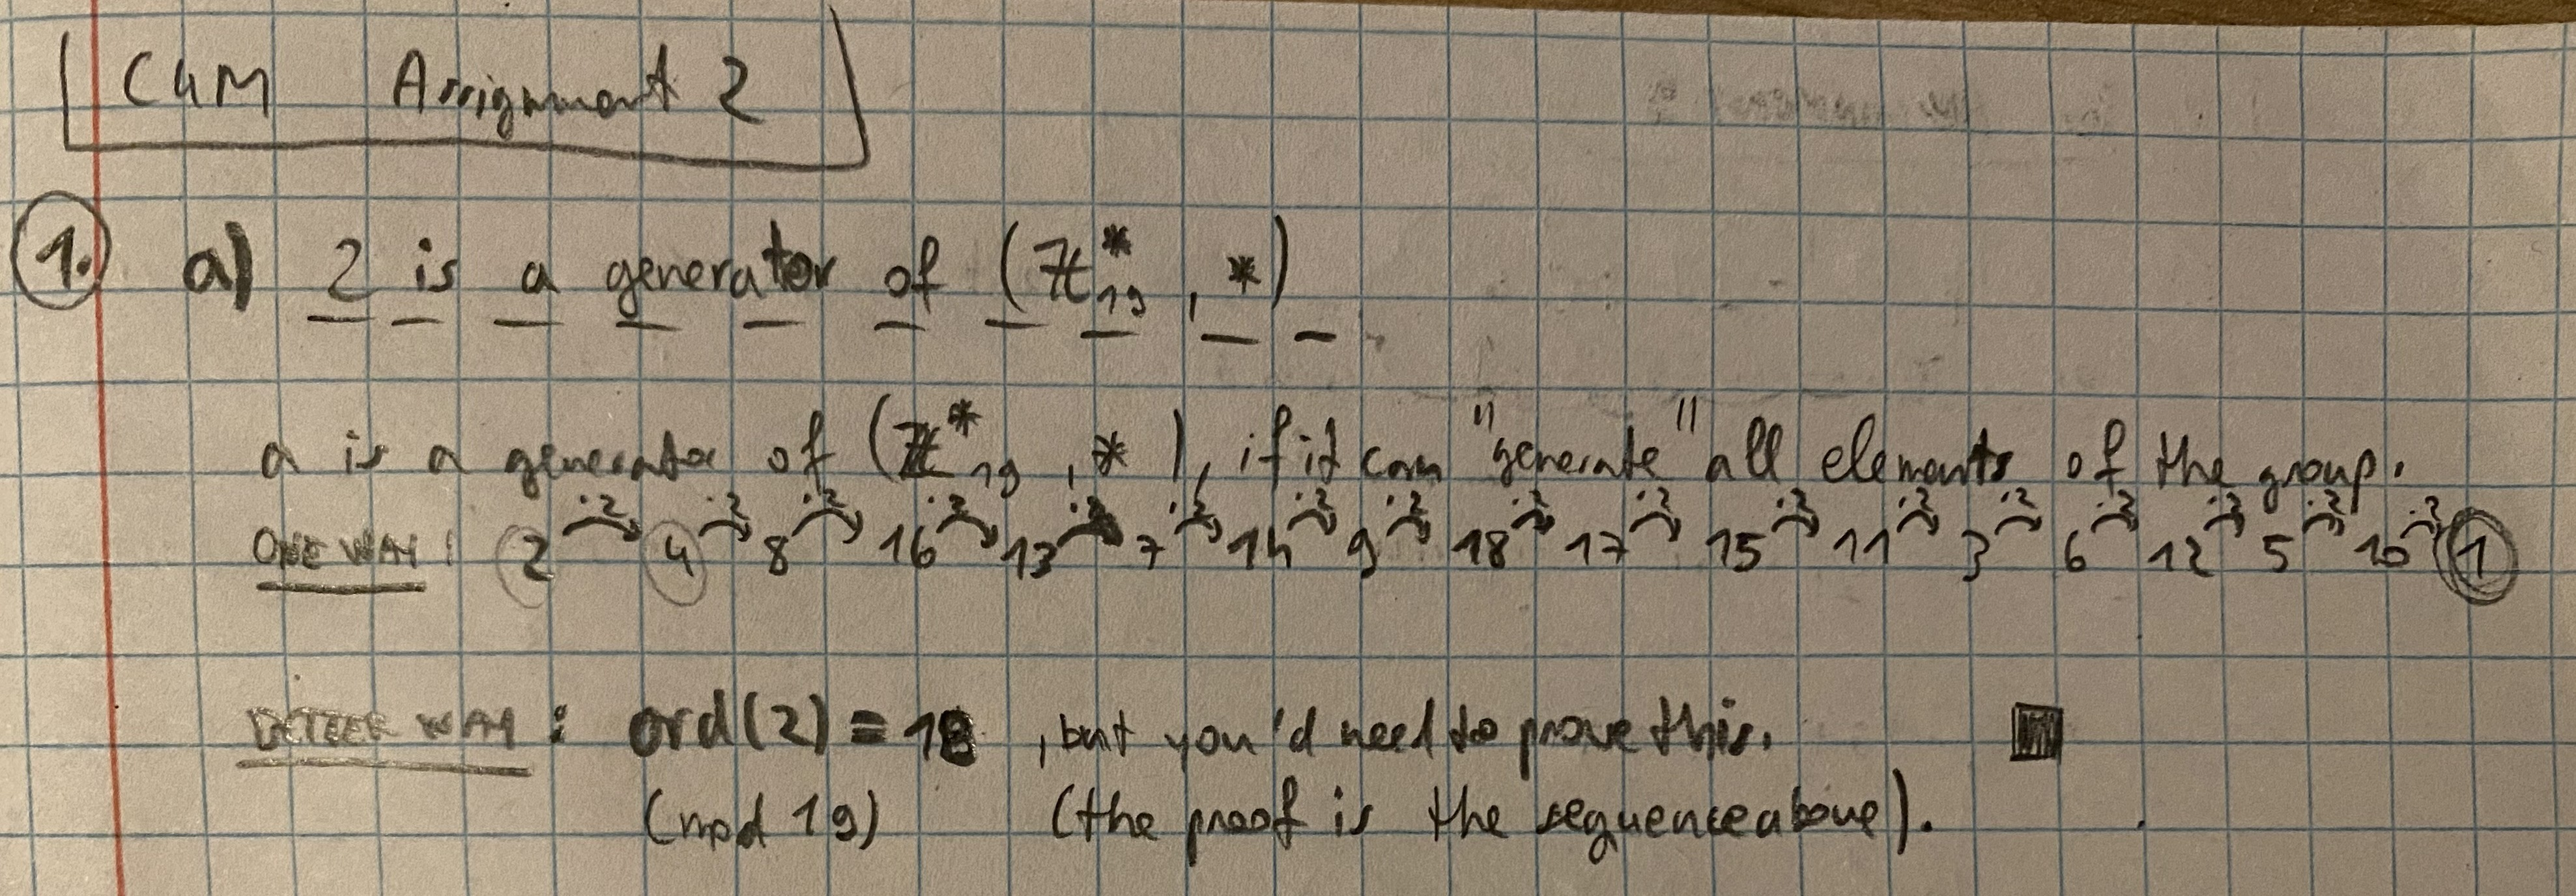
\includegraphics[scale=0.08]{1ex_a}
 \item Because 2 is a generator of the group $\mathbb{Z}_{19}$, every element is a power of 2 (mod 19). The elements in our group that have order 18 have to be elements that are powers of 2 and the power is coprime with 18. What I mean by that is if for example we want to see if 3 has order 18, we have to check how we get 3 from generator 2: $3 \equiv 2^{13}$ which means we can calculate powers of 3 with powers of 2, for example: $3^4 \equiv 2^{13 * 4}$. To get the order of 3, we need to find the smallest number k that will result in: $3^k \equiv 1$ which can be translated into: we need to find the smallest number k so that $18 | 13 * k$. Becuase 13 and 18 are coprime, our only option is $k = 18$.
 
 Following the same principle we can conslude that these elements (besides 2) have order 18: 3, 10, 13, 14, 15.

 \item If a group G has a prime order p (p number of elements), then the order of every element in the group has to be either 1 or the prime number p. This is because of the corollary after the Langrange's theorem states, that the order of any element in the group has to devide the number of elements in that group. Since p is prime (it's only devisible by 1 and p), all of the orders are either 1 or p. Since 2 is the lowest prime number, we have 2 or more elements. If all the elements were of order 1, they would all be equivalent to the identity element, which would mean that we only had 1 element (contradictory with the fact that we have 2 or more elements). Therefore at least one element has order p, which means that it generates the whole group, which means the group is cyclic.

\end{enumerate}

% -------------------------------------------------------------

\subsection*{Problem 2}
 
\begin{enumerate}[label= (\alph*)]

 \item 
\includegraphics[scale=0.107]{2ex_a}
 
 \textit{Deeper understanding}: If we want to check that $p$ is prime, we can only check the first few prime numbers that are smaller (or equal) than $\sqrt{p}$. The reason for this is that if $p$ is not prime (and $\sqrt{p} \notin{\mathbb{Z}}$) then p has at least 2 divisers $a, b \in \{2, 3, \ldots, p - 1\}$ so that $p = a b$. Both a and b cannot be larger than $\sqrt{p}$, since they would not multiply to p.

 \item Fermat's little theorem can't really help us in this case (or at least I don't see a useful connection). It tells us that $x^{556} \equiv 1 (\mod 557)$ for every integer x that isn't divisible by 557. 
 \item If I understood the question correctly then $x$ is an element of integers ($\mathbb{Z}$).
 \item 

\end{enumerate}

% ------------------------------------------------------------- 
\subsection*{Problem 3}
\begin{enumerate}[label= (\alph*)]

 \item We have a general formula $a + b \sqrt{5}$. This means that we can derive a and b from our examples: $-3 \sqrt{5} - 11 \implies a = -11, b = -3$. Let's chech the square: ${(-3 \sqrt{5} - 11)}^2 = 45 + 2 * 33 \sqrt{5} + 121 = 66 \sqrt{5} + 166 \implies a = 166, b = 66$.
 
 For our particular examples we can choose:
 $a1 = 2, b1 = 0 \implies ex_1 = 2,\\ a2 = 0, b2 = 2 \implies ex_2 = 2 \sqrt{5},
 a3 = -1, b = 1 \implies ex_3 = \sqrt{5} - 1$.

 From these definitions we can easily check that the sums and products still hold the same form. For example if we calsulate the sums and products of $ex_1$ end $ex_2$: $ex_1 + ex_2 = 2 \sqrt{5} + 2$ and $ex_1 * ex_2 = 4 \sqrt{5}$. The sums and products of the other two pairs is done in the same fashion.

 We can now make sure that the squares also hold shape:
 
 $ex_1^2 = 4 \implies a = 4, b = 0$; 
 $ex_2^2 = 20 \implies a = 20, b = 0$;

 $ex_3^2 = 6 - 2 \sqrt{5} \implies a = 6, b = -2$.

 \item 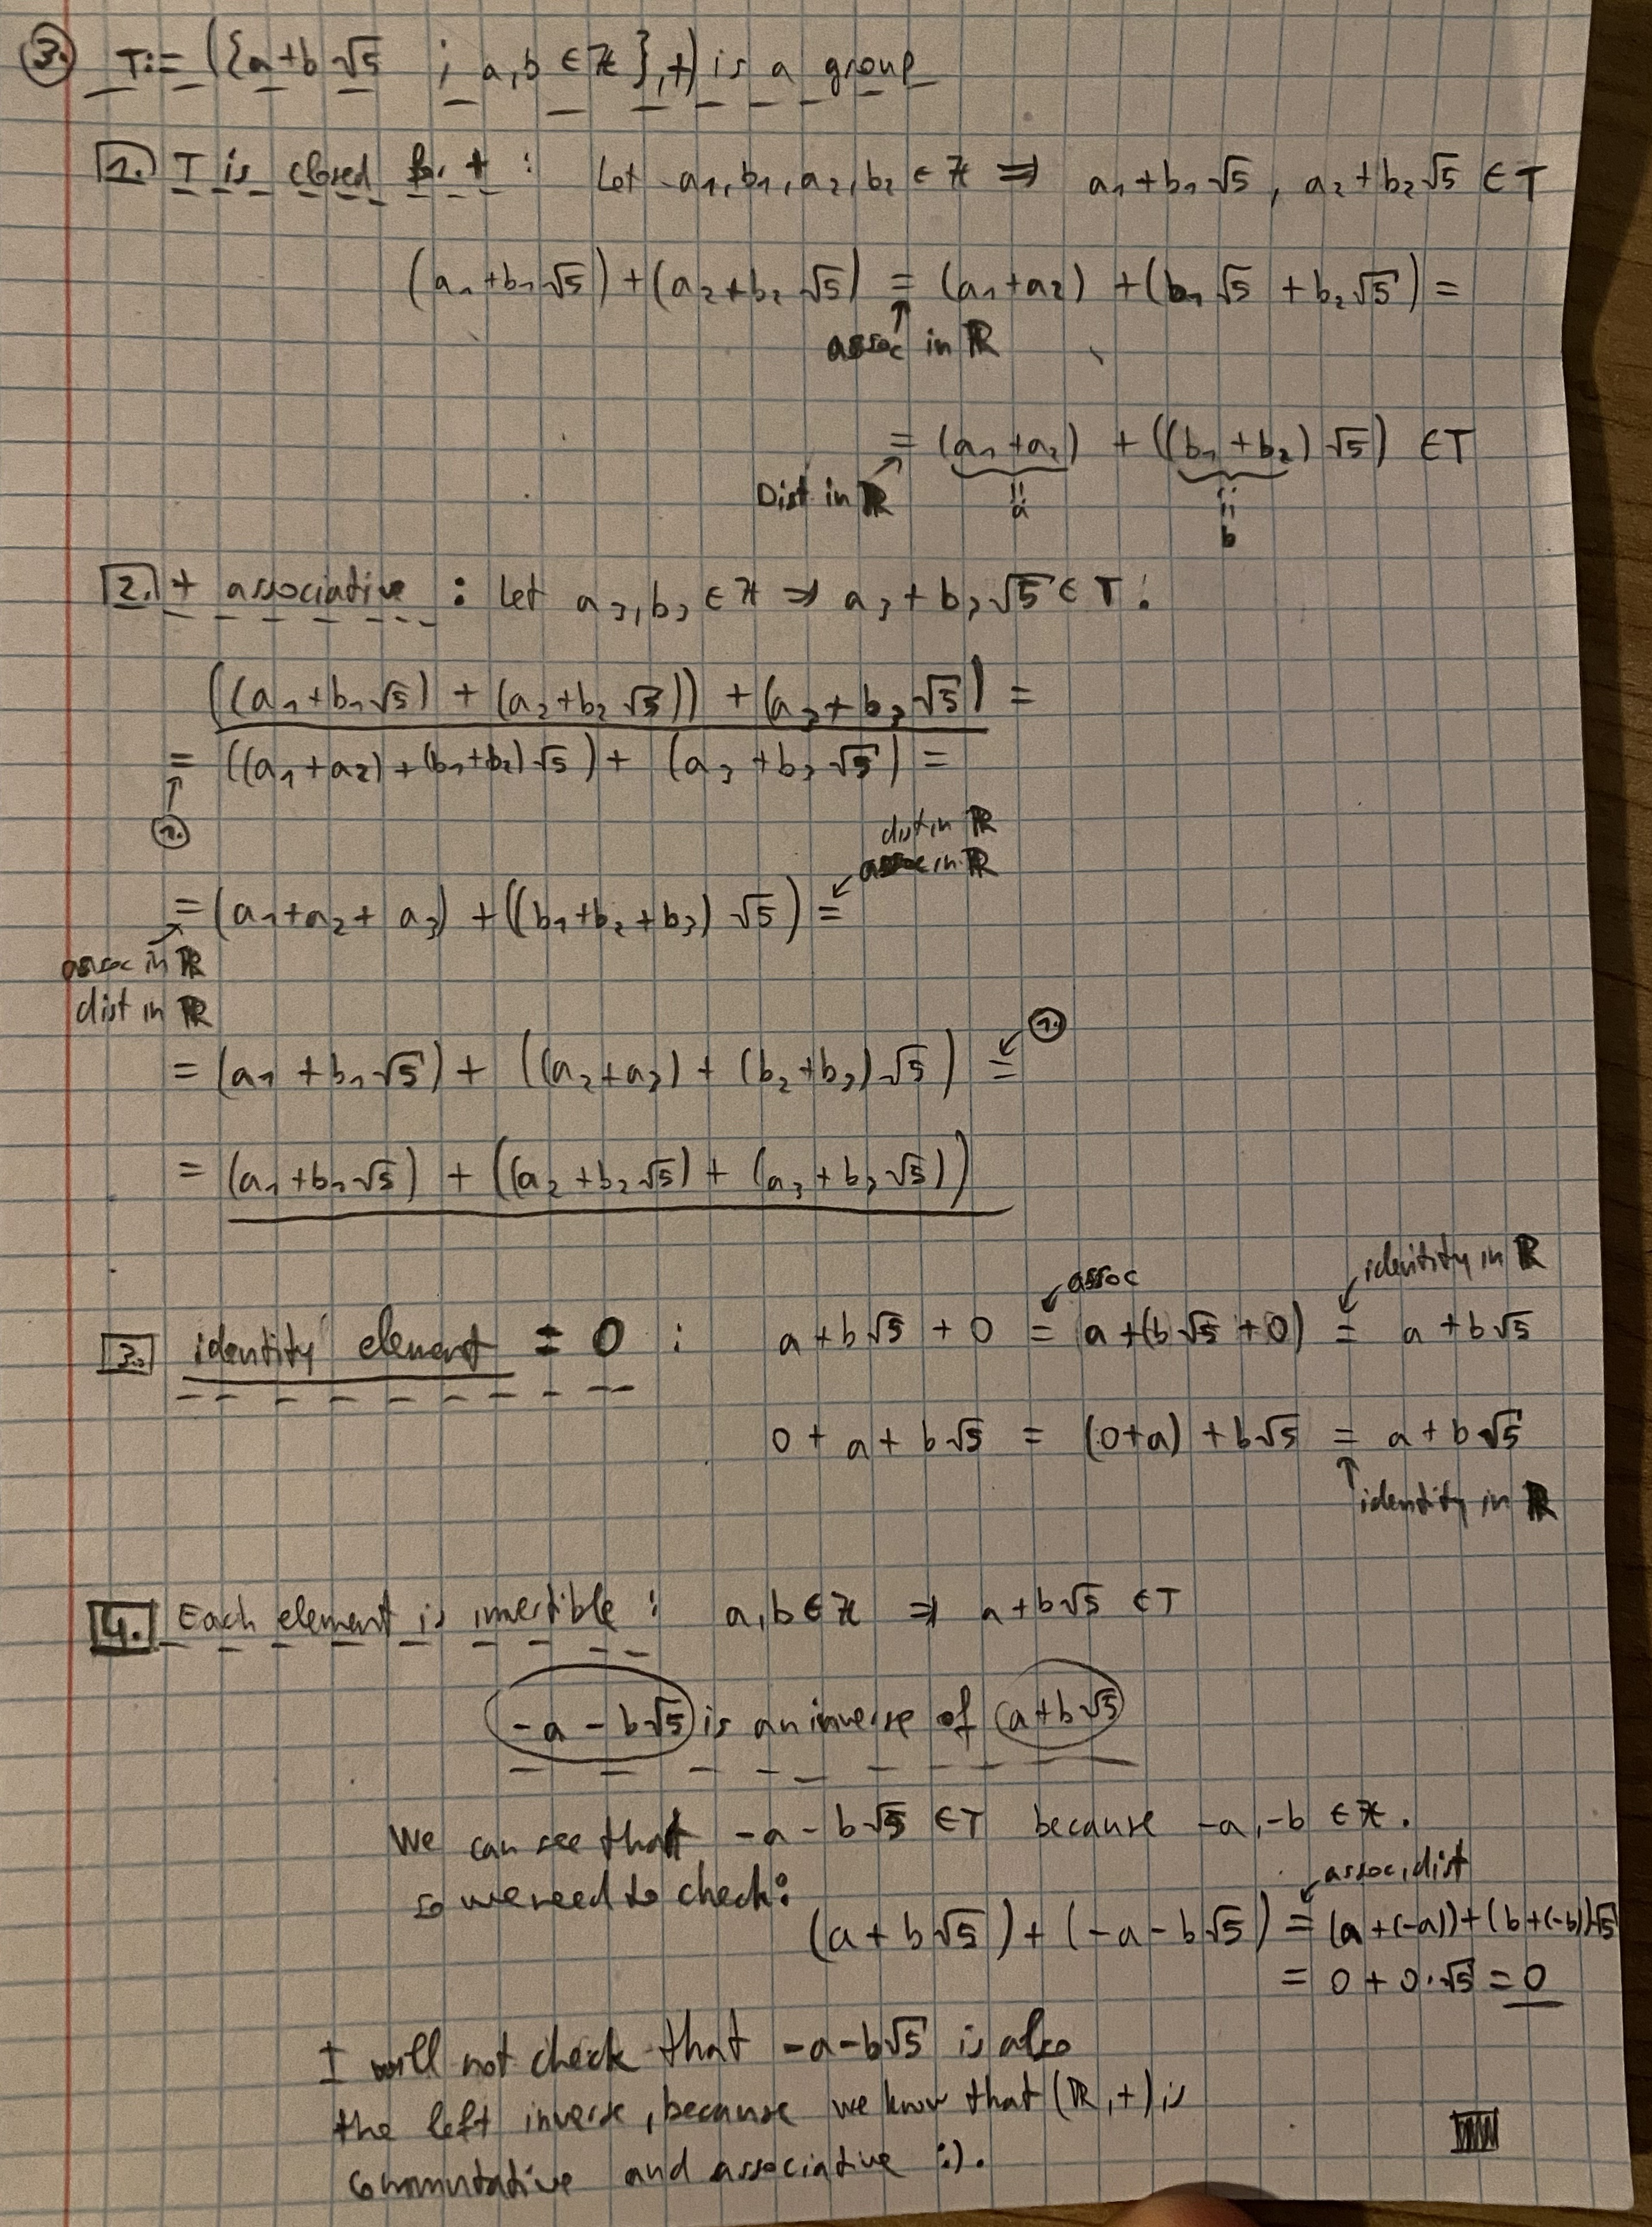
\includegraphics[scale=0.11]{3ex_b.jpeg}
 \item We can check that $(T, *)$ is closed and associative like we checked for addition. We can also check that the identity element for this group is 1.
 \item Generally (almost for all) an element of $(T, *)$ doesn't have an inverse. Here is a counter example:
 
 $(2 + 3 \sqrt{5}) * (x + y \sqrt{5}) = 1$

 $(2 * x + 3 * x * \sqrt{5} + 2 * y \sqrt{5} + 15 * y) = 1$

 $((2 x + 15 y - 1) + (3 x + 2 y)\sqrt{5}) = 0$

 but because the first parentheses belong to integers and the second parentheses doesn't, both have to be 0. If we solve the two equations we get: $x = \frac{-2}{41}, y = \frac{3}{41} \notin \mathbb{Z}$ which means that the element $2 + 3 \sqrt{5} \in (T, +, *)$ doesn't have an inverse in the group. Which further means that $(T, +, *)$ is not a field, only a ring.




\end{enumerate}

% -------------------------------------------------------------

\end{document}

